%\documentclass{jpsj3}
\documentclass[fp,twocolumn]{jpsj3}
%\documentclass[letter,twocolumn]{jpsj3}
%\documentclass[letterpaper,twocolumn]{jpsj3}
\usepackage{txfonts}
\usepackage{algorithm}
\usepackage{algorithmic}
\usepackage{amsmath}
\usepackage{multirow}

\usepackage{bm}
\usepackage{color}

\makeatletter
\@dblfptop 0pt
\makeatother

\renewcommand{\topfraction}{.85}
\renewcommand{\bottomfraction}{.60}
\renewcommand{\textfraction}{.15}
\renewcommand{\floatpagefraction}{.6}

\title{Derivaton of QUBO formulations for sparse estimation}

\author{Tomohiro Yokota$^1$%\thanks{jpsj{\_}edit@jps.or.jp}
  , Makiko Konoshima$^2$, Hirotaka Tamura$^2$, Jun Ohkubo$^{1,3}$}
\inst{$^1$Graduate School of Science and Enginnering, Saitama University,
  255 Shimo-Okubo, Sakura-ku, Saitama-shi, 338-8570, Japan\\
  $^2$Fujitsu Laboratories Ltd.,
  4-1-1 Kawasaki, Kanagawa 211-8558, Japan\\
  $^3$JST, PREST, 4-1-8 Honcho, Kawaguchi, Saitama 332-0012, Japan} %\\

\abst{
%(大久保)l1ノルムを提案するのなら propose the l1 norm でいいですが、l1ノルムのQUBO形式を提案するので、英語では順序が逆ですね。あと、他にもありうるので the ではなくて a がいいです。あとは、「見直すことによって変数を削減できた」という部分はもっと直接的に書いたほうがいいかもしれません。見直す、というよりも、〜の式を使って変数を削減、など。改訂案では単純に、変数を減らすことで単純化されたQUBO形式を得られた、という形にしてあります。

We propose a quadratic unconstrained binary optimization (QUBO) formulation of the $\ell_{1}$-norm, which enables us to perform sparse estimation in the Ising-type annealing methods including quantum annealing. The QUBO formulation is derived via Legendre transformation and the Wolfe theorem, which have recently been employed to derive the QUBO formulation of ReLU-type functions. Furthermore, it is clarified that a simple application of the derivation method gives a redundant variable; finally a simplified QUBO formulation is obtained by removing the redundant variable.

}

%%% Keywords are not needed any longer. %%%
%%% \kword{keyword1, keyword2, keyword3, \1dots} 
%%%

\begin{document}
\maketitle

\section{Introduction}

%(大久保)イントロはできるだけ丁寧に、厚みを持って、ですかね。なかなか難しいのですが・・。
In recent years, some novel computing hardwares have been developed and actually provided; 
there are some Ising-type annealing machines such as ``D-Wave 2000'' by the Canadian company D-Wave \cite{d-wave01,d-wave02} and ``FUJITSU Quantum-inspired Computing Digital Annealer'' by the Japanese company Fujitsu \cite{DA}. 
The annealing machines are used to obtain approximate solutions for optimization problems; the optimization problems play important roles in various research areas including data mining and machine learning.
Especially, the quantum annealing method has been originally proposed in \cite{Kadowaki1998}, and a similar idea called adiabatic quantum computing \cite{Farhi2001} has attract many attentions; recently, researches for practical applications have been performed (for example, see \cite{Tanahashi2019}.) 
Discussions for machine learning and quantum Boltzmann machines were given in \cite{Biamonte}, and there are many challenging tasks from the viewpoints of hardware and software. 
Although one of the restrictions are the small number of system size, the number of available qubits (or classical bits) has been increasing year by year, which enables us to tackle practical and large optimization problems.


%(大久保)最初の段落で現状の説明をして、でも〜という問題点があって、それについてどういう研究があって・・、ということを次の段落にしましょうか。あと、q-lossがなにか、なども読者はしらないので、その辺りの説明も少しはしておいた方が親切ですよね。

The above annealing hardwares need quadratic unconstrained binary optimization (QUBO) formulations; the hardwares are based on the Ising-type Hamiltonian, and hence it is necessary to convert original cost functions in optimization problems into the QUBO formulation. 
(The QUBO formulation is equivalent to the Ising model.)
Although continuous variable can be expressed as the Ising-type variables via adequate binary-expansions, in general, it is not straightforward to reformulate the original cost functions as the QUBO formulation.
Some reformulations were given in \cite{Lucas2014}, and it has been shown that logic gates are expressed in the form of the QUBO formulations.
However, a systematic way to derive the QUBO formulations has not been found yet.
Recently, the Legendre transformation was employed to derive the QUBO form of the $q$-loss function \cite{q-loss}; 
the $q$-loss function was proposed as a cost function with robust characteristics against the label noise in machine learning. 
The derivation technique based on the Legendre transformation revealed that some mathematical transformation would be needed to transform some types of cost functions into the QUBO form.
Actually, it has been clarified that the Legendre transformation is not enough to deal with the Rectified Linear-Unit (ReLU) type functions \cite{relu};
the Wolfe duality theorem \cite{wolfe} was employed to derive the QUBO form for the ReLU-type functions.
These works also indicate the fact that the derivation of the QUBO formulations is not straightforward, and we sometimes needs further considerations depending on the original cost functions.



%(大久保)文章のつながりを少し意識してみました。q-lossは機械学習のためのものですし、ReLUは、まあIMRT向け、だったのですが、とりあえずは機械学習でよく使われる、と考えて、そうではないものもありますよね? データマイニングとかで、スパース制約を考える必要もあって、l1はその一つですよね?という流れ。いかがでしょうか? あと、ブラックホールのところで「we performed」とあるのですが、我々はやっていないので・・(笑)。

As shown above, there are some works to derive the QUBO formulation for machine learning problems.
Of course, there are many other research fields related to optimization problems, and one of them is data analysis and data mining.
It has been known that regularization plays an important roles in data analysis and, of course, machine learning.
$\ell_{2}$ norms are widely used; for example, a linear regression with the $\ell_{2}$ regularization is called the ridge regression.
$\ell_{1}$ norms are used in order to introduce a kind of sparseness;
the sparse estimation is one of hot topics in the research field of data analysis.
Least absolute shrinkage and selection operator (LASSO) \cite{lasso} is a famous practical method to achieve sparse estimations, in which the $\ell_{1}$ norm is added to a least-squares cost function.
The idea of the sparse estimation was also applied to the recent black hole analysis \cite{black-hole}.
The black hole is so small that it is difficult to observe it because of the low-resolution of images.
Therefore, simultaneous measurements from radio telescopes all over the world are performed,
and the method based on the sparse estimation is applied to the observed big data, by which only essential information is extracted and finally the imaging of the black holes was achieved.
Note that $\ell_{2}$ norm is simply connected to the QUBO formulation because of the quadratic form; 
in contrast, $\ell_{1}$ norm has a non-differentiable point, and the QUBO formulation has not been derived yet.


%(大久保)できるだけ受動態で、というのが学術論文の基本なので、そんな感じに書き直してみました。あと、意義をもう少し主張するために、単純な適用だけでも駄目、という部分を少し強調する形にしてみました。ちょっと弱いんですけど・・。

In this paper, the QUBO form of the $\ell_{1}$ norm is derived.
In order to obtain the QUBO formulation, both the Legendre transformation and the Wolfe duality theorem are employed.
Furthermore, it is clarified that only the simple applications of the previous derivation techniques are not enough;
through numerical checks and reconsidering the derived formulation, a simplified QUBO formulation is finally derived.
The reduction of the number of variables is important for the hardware implementation 
because the current Ising-type hardwares have only restricted number of qubits (or classical bits).


%(大久保)Section * ... のように、Sectionがすべて主語になると、ちょっと単調なので書き直してみました。
The construction of this paper is as follows.
Section~2 explains the QUBO form, previous works.
The important technique and theorem are also given for later use in the derivation.
In Sect.~3, the QUBO form of the $\ell_{1}$ norm is derived,
and the numerical checks are given.
Section~4 gives the main result of this paper;
a simplified version of the QUBO form is given,
in which a variable is removed from the QUBO form in Sect.~3.
Section 5 gives concluding remarks and future works.


\section{Backgrounds and preliminaries}
In this section, we describes the knowledge.

%(大久保)直訳するとこんな感じかも、ですが、論文では見たことのない表現では?? 以下のような感じではいかがでしょうか? あと、セクション名も簡潔すぎるので変えました。
In this section, some background knowledge and previous works are briefly denoted.


\subsection{QUBO and Ising model} %QUBOとIsingモデルについての説明
Since the QUBO formulation and the Ising model are equivalent, we can be converted to other form if we can be represented one side. The Ising model is represented as follows:

%(大久保)少し導入も追加してみました。
As denoted in the Introduction, the Ising-type annealing machines need the Ising Hamiltonian or the QUBO formulation in order to solve combinatorial optimization problems. 
The QUBO form has binary variables, which take only $1$ or $0$, and the $0$-$1$ binary variables are sometimes suitable to consider the combinatorial optimizations; some problems are formulated as integer programming problems, or problems with continuous variables can be treated by the usage of the binary expansions. 
Of course, since the QUBO formulation and the Ising model are equivalent, it is possible to convert the QUBO form into the Ising model, and vice versa.
The Ising model is represented as follows:

\begin{eqnarray}
  H=-\sum_{i,j}{J_{i,j}\sigma_{i}\sigma_{j}}-\sum_{i}{h_{i}\sigma_{i}}
\end{eqnarray}
where $\sigma_{i}\in \{-1,+1\}$is a spin variable for $i$-th spin, $J_{ij}\in \mathbb{R}$ a quadratic term of $i$ and $j$, and $h_{i}\in \mathbb{R}$ a liner term of $i$. We can easily converted the Ising model to QUBO formulation, which uses binary variable $q_{i}\in \{0,1\}$, by applying $q_{i}=\frac{\sigma_{i}+1}{2}$ and QUBO formulation is represented as follows:

%(大久保)J_ij は「quadratic term」ではなくて、係数、ですよね。そのあたりも書き直して、以下のような感じはいかがでしょうか? あと、本文中だと分数は \frac を使うとフォントが小さくなって見づらいので、スラッシュで書くことが多いです。
\noindent
where $\sigma_{i} \in \{-1,1\}$ is a spin variable for $i$-th spin, $J_{ij}\in\mathbb{R}$ a coefficient related to a quadratic term between spin $i$ and $j$, and $h_{i}\in\mathbb{R}$ a coefficient for a linear term with spin $i$.
Let $q_{i} \in \{0,1\}$ be a binary variable corresponding to the $i$-th spin,
and then by applying the variable transformation $q_{i}=(\sigma_{i}+1)/2$,
we have

\begin{eqnarray}
  H=-\sum_{i,j}{\widetilde{J}_{i,j}q_{i}q_{j}}-\sum_{i}{\widetilde{h}_{i}q_{i}},
\end{eqnarray}
%(大久保)数式の後ろはピリオドかカンマをつけましょう(英語ではそうします)。カンマを追加しておきました。さらに、以下を追加。記号の説明もないですしね。
where $\widetilde{J}_{i,j}$ and $\widetilde{h}_{i}$ should be transformed from $\{J_{ij}\}$ and $\{h_{i}\}$ adequately.
As for the relations between the QUBO formulation and the Ising Hamiltonian, please see Ref.~\citen{Tanahashi2019};
in Ref.~\citen{Tanahashi2019}, some examples of the QUBO formulations for typical optimization problems are also given.



%(大久保) q-loss の導出にLegendreを使うので、先に述べておく形にしてみました。節を追加。

\subsection{Legendre transformation}

For reader's convenience, we here give a brief notation for the Legendre transformation.

If a function $f_{L}$ is convex, the Legendre transformation of $f_{L}$, the so-called conjugate function of $f_{L}$, is given as follows:
\begin{align}
\label{eq:Legmax}
f_{L}^{*}(t)=\sup_{x}\{t x - f_{L}(x)\}.
\end{align}
That is, the variable $t$ is introduced, and the function for $x$ is transformed to the function for $t$.
In addition, \eqref{eq:Legmax} is equivalent to following equation:
\begin{align}
\label{eq:Legmin}
f_{L}^{*}(t)=-\inf_{x}\{f_{L}(x) - t x\}.
\end{align}


\subsection{Previous work 1: $q$-loss function}

%(大久保)もう少し節を細かく分けてみましょうか。q-loss と ReLU をわけて、あとはそれらで使った Legendre の定義も書いてみる、など。節のタイトルを変えました。
Here, a brief review of the previous work by Denchev \textit{et al.} is given \cite{q-loss}.
the following $q$-loss function was proposed in Ref.~\citen{q-loss}:

\begin{eqnarray}
  L_{q}(m)=\min{[(1-q)^{2}, (\max{[0,1-m]})^{2}]} \label{q-loss_function}
\end{eqnarray}

%(大久保)もう少し q-loss についての説明も追加しておきましょうか。
\noindent
where $q \in (\infty,0]$ is a parameter and $m$ is a continuous variable. 
In Ref.~\citen{q-loss}, there is a discussion for the application of the $q$-loss function in machine learning problems, and the $q$-loss function has a robust features against label noise.
Since Eq.~\ref{q-loss_function} has a $\max$ function, it is not easy to see the QUBO form of the $q$-loss function.
Denchev \textit{et al.} employed the Legendre transformation,
and finally the following function was derived\cite{q-loss}:

\begin{eqnarray}
  L_{q}(m)=\min_{t}{\left\{(m-t)^{2}+(1-q)^{2}\frac{(1-\text{sign}(t-1))}{2}\right\}}, \label{q-loss_function_legendre}
\end{eqnarray}
%(大久保)数式の後ろにピリオドかカンマ。ここではカンマ。変数$t$が出てきたので、説明しておきましょう。

where $t$ is an additional variable which is introduced via the Legendre transformation.
Although the variables $m$ and $t$ in Eq.~\eqref{q-loss_function_legendre} are continuous, the usage of the binary expansions gives the QUBO formulation for the $q$-loss function.
As for details of the binary expansions, please see Ref.~\citen{q-loss}.
Note that the sign function in Eq.~\eqref{q-loss_function_legendre} is also expressed as a one-body term when we employ the binary expansion.


%(大久保)Wolfeを ReLU の前にもってきました。流れ的に、先に紹介しておいた方がいいかな、と。あと、ここだけは入れ替えたこともあって、もとの文章を残さずに、赤文字だけにしてあります。あと、数式の下付き添え字は、変数なら italic ですが、文字なら non-italic です。あと、多変数にしておきました。Legendreの方は1変数なんですけど・・。

\subsection{Wolfe-duality} \label{sec:wolfe}
In nonlinear programming and mathematical optimization, the Wolfe duality theorem\cite{wolfe} is used to convert a main problem with inequality constraints to a dual problem.
For a differentiable objective function and differentiable constraints, 
the main problem is written as follows:
\begin{equation}
  \left\{ \,\,
  \begin{aligned}
    & \text{minimize}_{\bm{x}}  \quad  f_{\mathrm{W}}(\bm{x}) \quad \quad \ (\bm{x} \in \mathbb{R}^{n}),\\
    & \text{subject to}  \ \quad h_{i}(\bm{x})\leq 0 \quad (i=1,2,\dots,l). \label{object_function}
  \end{aligned}
  \right.
\end{equation}
where $f_{\mathrm{W}}(\bm{x})$ is a certain convex function to be optimized and $h_{i}(\bm{x})$ are convex and inequality constraints. The Lagrangian function for this optimization problem is
\begin{eqnarray}
  L(\bm{x},\bm{z})=f_{\mathrm{W}}(\bm{x})+\bm{z}^{T}h(\bm{x}),
\end{eqnarray}
where $\bm{z}$ is a vector of the Legendre coefficients. 
Then, the Wolfe dual theorem means that the minimization problem in Eq.~\eqref{object_function} in equivalent to the following maximization problem:
\begin{equation}
  \left\{\,\,
  \begin{aligned}
    & \text{maximize}_{\bm{x},\bm{z}}  \quad L(\bm{x},\bm{z}) \quad \quad \quad \ ((\bm{x},\bm{z})\in \mathbb{R}^{n}\times\mathbb{R}^{l}),\\
    & \text{subject to}  \qquad \nabla L(\bm{x},\bm{z})=0 \quad (\bm{z} \geq 0).
  \end{aligned}
  \right.
\end{equation}
As shown above, the Wolfe dual theorem transforms the minimization problem to the maximization problem.


%(大久保)節を追加しました。
\subsection{Previous work 2: ReLU-type function}
\label{sec:ReLU}

%(大久保)適切な引用をしつつ、ですかね?
In Ref.~\citen{relu}, the QUBO form of the following ReLU-type function was discussed:

\begin{eqnarray}
  f_{\mathrm{R}}(m)=-\min{(0,m)}. \label{ReLU_function}
\end{eqnarray}
%(大久保)数式にピリオドを追加しました。あと、関数 f はこのあと使うので、下付き添え字をつけておきました。

%(大久保)書くなら as follows: ですかね? 受け身形を使いつつ、英語を少し整えました。
\noindent
Note that the function $f_{\mathrm{R}}(m)$ becomes the conventional ReLU function when the variable transformation $m \to -m$ is employed.
As shown in Ref.~\citen{relu}, a naive application of the Legendre transformation to the function $f(m)$ in Eq.~\eqref{ReLU_function} gives the following expression:

\begin{eqnarray}
  f_{\mathrm{R}}(m)=-\min_{t}{\{-mt\}} \quad \text{subject to} \quad -1\leq t\leq 0, \label{ReLU_function_legendre}
\end{eqnarray}

%(大久保)カンマを追加。また、やはり新しい記号の説明。
\noindent
where $t$ is a new variable which stems from the Legendre transformation.

%(大久保)英語を整えてみました。あと、次の section にマイナスサインのことが数式で記述されていますが、こっちに書いた方がわかりやすいのでは? ということで以下のような形ではいかがでしょうか?

Although Eq.~\eqref{ReLU_function_legendre} has the QUBO form, it is not suitable for optimization problems.
This is because the minus sign before the $\min$ function;
when the ReLU-type function is used as a kind of constraints or penalty terms for an optimization problem with a cost function $C(m)$, the whole minimization problem is, for example, given as follows:
\begin{eqnarray}
  \min_{m} \left\{ C(m)+f_{\mathrm{R}}(m) \right\} &=& \min_{m}\left\{ C(m)-\min_{t} \{-mt\} \right\} \nonumber \\
  &\neq& \min_{m,t} \left\{C(m)-(-mt)\right\} ,
\end{eqnarray}
and hence the cost function $C(m)$ and the ReLU-type function $f_{\mathrm{R}}(m)$ cannot be minimized simultaneously.
Therefore, the Wolfe duality theorem was employed in Ref.~\citen{relu}, and finally the following formulation was derived:
\begin{eqnarray}
  f_{\mathrm{R}}(m)=\min_{t,z_{1},z_{2}} \left\{mt+z_{1}(t+1)-z_{2}t-M(-m-z_{1}+z_{2})^{2}\right\} \label{ReLU_function_wolfe}
\end{eqnarray}
where $M$ is a large positive constant. 
It is easy to see that Eq.~\eqref{ReLU_function_wolfe} can be used with the combination of the cost function $C(m)$.



\section{Naive derivation of QUBO formulation for $\ell_{1}$-norm} \label{Native_derivation}
In this section, we derive the QUBO formulation of absolute function.

%(大久保)もう少し説明を加えてみました。次の節との違いも出したいので。

In this section, the Legendre transformation and the Wolfe dual theorem are applied to the $\ell_{1}$ norm-type function naively. 


\subsection{QUBO formulation}


\begin{figure}[tb]
  \begin{center}
    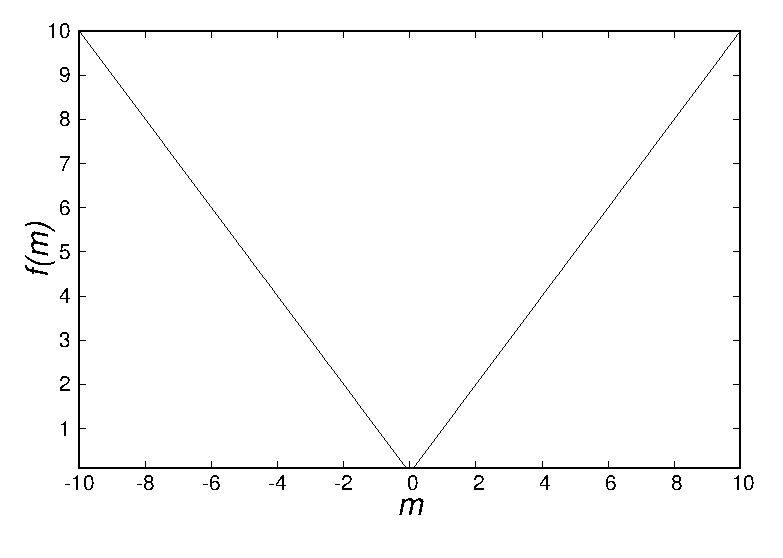
\includegraphics[keepaspectratio,scale=0.50]{absolute.eps} \\
    \begin{minipage}{0.03\hsize}
      \vspace{2mm}
    \end{minipage}
    %(大久保)元が「Outline of l1-norm」だったのですが、\ellを使うとか体裁を。少し変更しました。
    \caption{$\ell_{1}$-norm in Eq.~\eqref{l1-norm}}
    \label{fig:absolute}
  \end{center}
\end{figure}

%(大久保)この部分なのですが、まずは絶対値関数という説明から入りましょうか。あと、素朴にReLUタイプ関数を使えばできるわけですが、それだと変数の数が多くて、というのも書いておいて、だから変数を減らすのが大切そう、という感じで次に繋げてみるのはいかがでしょうか? 数式の上の文章を以下のような感じに。

Although the $\ell_{1}$-norm is usually denoted as an absolute value of a variable, i.e., $\lvert m \rvert$, here we employ the following function $f(m)$:\\
\begin{eqnarray}
  f(m)=-\min{\{-m,m\}} \label{l1-norm}
\end{eqnarray}


%(大久保)で、そのあとに説明を追加。このあたりからこの論文のメインなんですが、かなり簡潔に書きすぎているので、しっかりと書く形にします。短すぎるのはあんまりよくないので。

Note that $f(m)$ can be expressed as follows:
\begin{eqnarray}
f(m)=-\min{\{0,m\}} - \min\{-m,0 \} = f_{\mathrm{R}}(m) + f_{\mathrm{R}}(-m),
\end{eqnarray}
where $f_{\mathrm{R}}(m)$ is the ReLU-type function in Eq.~\eqref{ReLU_function}.
Hence, it is easy to obtain the QUBO formulation for $f(m)$ by using the discussion based on Sect.~\ref{sec:ReLU}.
However, the QUBO formulation needs six additional variables.
The derivation below enables us to obtain the QUBO formulation for $f(m)$ with only three additional variables.



A function form of $f(m)$ in shown in Fig. \ref{fig:absolute}. And by applying the Legendre transrormation to the function $f(m)$ in (\ref{l1-norm}), we can transform it as follow. 
\begin{eqnarray}
  F(m)=-\min_{t}{\{-mt\}} \quad \text{subject to} \quad \-1 \leq t \leq 1 \label{legendre}
\end{eqnarray}

%(大久保)このLegendre変換もそんなに自明なものではないですよね? 佐藤さんの論文では、場合分けをしつつ、この導出をしっかりと書きました。前の節にLegendre変換についても記載したことですし、佐藤さんの論文と同じような感じでこの導出を詳しく書いてもらえますか? もし図を入れた方がわかりやすいな、と思えば図を入れてもいいですし。あまりに結果が簡潔すぎるので、もう少しきちんと書くことにしましょうか。あと、Legendre変換を2回するので、もとの関数に戻るわけですが、それだと f(m) と書くべき、なんです。でも、二次形式ですよ、ということを明示するために、佐藤さんの論文では F(m) のように記号を変えました。ここでもそのために記号を変えているはずですが、唐突に F(m) が出てきて、説明もないので、理解できないかな、という感じ。佐藤さんの論文を参考にしつつ、記号の説明の追記もお願いします。

{\color{red}
  (more explanation...)
  ルジャンドル変換は関数f(x)から別の関数g(p)を導く変換である. ここで, 関数f(x)が凸関数である場合, 関数g(p)に対してルジャンドル変換を適用することで元の関数f(x)に戻る特性がある. しかし, ルジャンドル変換を二回適用することで導出される関数は二次形式となるため, ここではF(m)と表記する.
}


%(大久保)この上の部分は前節に移しましたので、不要です。軽く触れるくらいにしましょう。Legendreのところの追記をする予定なので、文章の流れをそれに合わせます。なので、その追記を見て、ですが、例えば下記のような感じになるのかな、と思います。

As shown in Sect.~\ref{sec:ReLU}, although the obtained expression via the Legendre transformation has a quadratic form, it cannot be combined with another cost function.
Hence, the Wolfe dual theorem is employed;
the following expression is immediately obtained by applying the Wolfe dual theorem to $F(m)$:

\begin{eqnarray}
  \widetilde{F}(m)=\max_{t,z_{1},z_{2}} \{-mt-z_{1}(t+1)+z_{2}(t-1)\} \label{wolf}
\end{eqnarray}
\begin{equation}
  \text{subject to} \quad \left\{
  \begin{aligned}
   -m-z_{1}&+z_{2}=0, \nonumber \\
   \ -1\leq t\leq 1, & z_{1}\geq 0, z_{2}\geq 0. \nonumber \\
  \end{aligned}
  \right.
\end{equation}

%(大久保) following penalty term とあるのですが、次のようなペナルティ項、と言いつつ、いきなり最終的なコスト関数の形が出てくるので文章としておかしいです・・。

This reformulation has the equality constraint, $-m-z_{1}+z_{2}=0$; in order to embed this constraint into the QUBO formulation, it is enough to add the squared term as a penalty. 
Therefore, the optimization problem (\ref{wolf}) can be represented as follows:

\begin{equation}
  \begin{aligned}
    \widetilde{F}(m)&=\min_{t,z_{1},z_{2}}{\{mt+z_{1}(t+1)-z_{2}(t-1)} \\
    &\quad+M(-m-z_{1}+z_{2})^{2}\} \label{after_wolf} \\
  \end{aligned}
\end{equation}
\begin{eqnarray}
  \text{subject to} \quad -1\leq t\leq 1, z_{1}\geq 0, z_{2}\geq 0, \nonumber
\end{eqnarray}

%(大久保)文章が長いので、少し変更。あと、スペルミスも多いかな・・。

\noindent
where $M$ is a constant and takes a large value to ensure the equality constraint, $-m-z_{1}+z_{2}=0$, to be satisfied.
Note that there are remaining inequality constraints, $-1\leq t\leq 1, z_{1}\geq 0$, and $z_{2}\geq 0$;
these inequality constraints can be easily realized by expanding these variables $t,z_{1}$, and $z_{2}$, in the binary expressions which satisfy the corresponding domain constraints respectively.

As a result, the QUBO formulation for the $\ell_{1}$-norm is expressed by using additional three variables.

\subsection{Numerical validation}

%(大久保)略語をいきなり出さない、など、あれこれと修正してみました。SAは略さないほうが一般的かな、と思います。

Here, numerical checks are given in order to see the validity of the obtained QUBO formulation in Eq.~\eqref{after_wolf}. We expect that the QUBO formulation will be used within quantum annealing methods or simulated annealing methods, and here simulated annealing algorithms are employed.
Since he purpose here is to verify the obtained QUBO formulation, the function in Eq.~\eqref{after_wolf} is experimented with continuous variables without binary expansions. 

%(大久保)箇条書きで書く必要もないかな、と・・。あと、constant m と書いておきつつ、直後に乱数で、というのも(わかるんですけど)誤解されると思います。あと、実験は何回やりました?? 書かれていなかったので・・。

The aim here is to check whether $\widetilde{F}(m)$ in Eq.~\eqref{after_wolf} gives the $\ell_{1}$-norm in Eq.~\eqref{l1-norm}. 
We randomly generate $m$ and check the value of $\widetilde{F}(m)$ by using a simulated annealing method for continuous variables. $m$ is chosen from a uniform distribution in the range of $[-10,10]$. 
The numerical experiments are performed (??? number) times.
In each numerical experiments, the initial conditions for the additional variables, $t, z_{1}$, and $z_{2}$ is chosen as follows:
\begin{itemize}
\item $t$ is generated from an uniform distribution with the range of $[-1,1]$.
\item $z_{1}$ and $z_{2}$ are generated from an uniform distribution with the range of $[0,10]$.
\end{itemize}


%(大久保)まあ、箇条書きじゃなくていいかな、と・・。

As the simulated annealing method for the continuous variables, we employ a conventional Metropolis-Hastings-type method.
In order to generate next candidates of the state, each variable moves by the amount of $+0.001$ or $-0.001$ with the same probability for each iteration.
At each iteration, the temperature is changed with the annealing schedule $T_{n+1}=0.9999T_{n}$, where $n$ is the iteration step.
The initial temperature is set as 
As for the annealing procedures, $T_{1}=1000$, and the annealing is finished when the temperature is lower than  $10^{-3}$.


%(大久保)図では tilde F ではなくて F' になっているんですけど、なぜ?? ここはチルダのままで行きましょう。あと、そもそもプライム(ダッシュ)は微分の意味を持つので、使いたくないです・・。

\begin{figure}[tb]
  \begin{center}
    \begin{tabular}{c}
      \begin{minipage}{0.50\hsize}
        \centering
        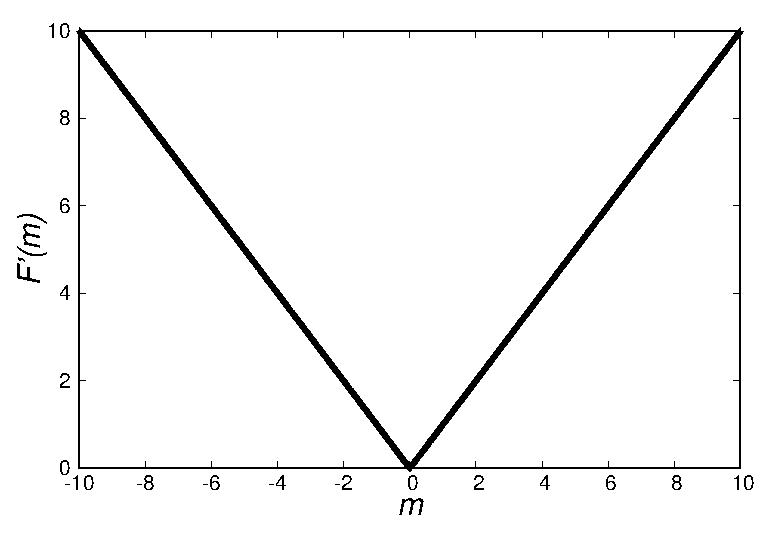
\includegraphics[keepaspectratio,scale=0.33]{minimum_cost.eps}
      \end{minipage}
      \begin{minipage}{0.50\hsize}
        \centering
        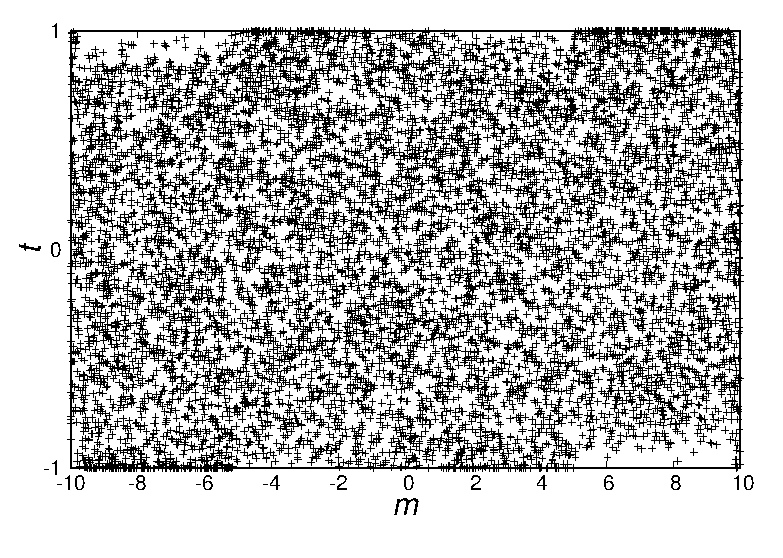
\includegraphics[keepaspectratio,scale=0.33]{minimum_t.eps}
      \end{minipage} \\
      \begin{minipage}{0.50\hsize}
        \centering
        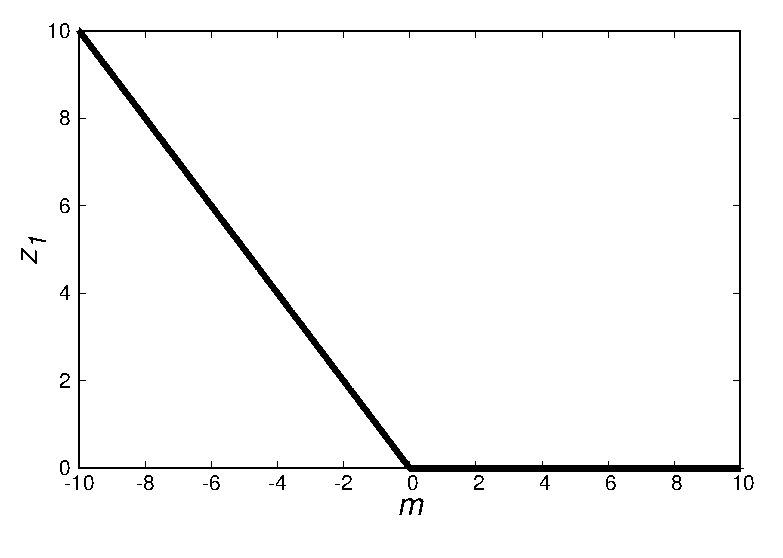
\includegraphics[keepaspectratio,scale=0.33]{minimum_z1.eps}
      \end{minipage}
      \begin{minipage}{0.50\hsize}
        \centering
        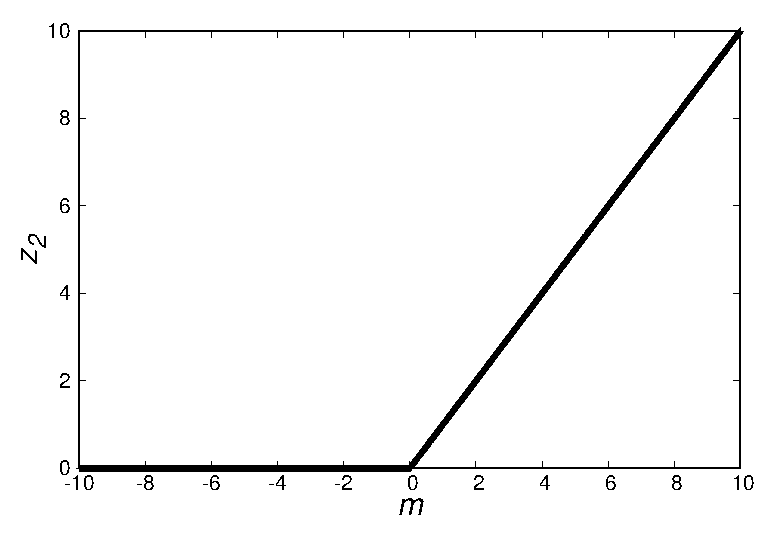
\includegraphics[keepaspectratio,scale=0.33]{minimum_z2.eps}
      \end{minipage}
    \end{tabular}
    \begin{minipage}{0.03\hsize}
      \vspace{2mm}
    \end{minipage}
    \caption{%(大久保)英語の論文の図のキャプションは、最初は文章ではなくて、説明の単語(?)だけ、が一般的なので、書き直してみました。
Numerical results obtained from the annealing method. $m$ is chosen randomly, and the annealing is performed; each $m$ gives a value of $\widetilde{F}(m)$. The values of $t, z_{1}, z_{2}$ at the optimum states are also shown.

}
    \label{fig:minimum1}
  \end{center}
\end{figure}

%(大久保)図を本文中に引用していないので、追記。他、少し書き直し。

Figure~\ref{fig:minimum1} shows the results of the annealing.
We confirm that $\ell_{1}$-norm is adequately recovered by the optimization of Eq.~\eqref{after_wolf}.
Not only the value of the cost function $\widetilde{F}(m)$, but also the values of the three additional variables are also shown in Fig.~\ref{fig:minimum1};
it is clear that $z_{1}$ and $z_{2}$ converge to specific values, but $t$ takes various values randomly. 
This means that $t$ would not be necessary for the optimization, which may give us a further simplified QUBO formulation for the $\ell_{1}$-norm.


\section{Reduced QUBO formulation} %定式化の見直し
\subsection{Reduction of the variable in the Legendre transformation}


%(大久保)もう少し丁寧に書いてみました。

As discussed above, the naive application of the Legendre transformation and the Wolfe dual theorem gives the QUBO formulation with three additional variables.
However, from the numerical experiments in the previous section, it is revealed that the variable $t$, which stems from the Legendre transformation, may not be necessary for the optimization problem.
Because of the restriction of the number of spin variables, it is preferable to have smaller number of variables in general.
Hence, here we try further reduction of variable from the QUBO formulation in Eq.~\eqref{after_wolf}. 

In order to achieve the elimination of $t$ from Eq.~\eqref{after_wolf}, we focus on the equality constraint $-m-z_{1}+z_{2} = 0$.
By employing the equality $z_{2} = m+z_{1}$, we have 

%(大久保)F'(m)としてあったのですが、プライム(ダッシュ)は微分の意味合いなので避けましょうか。ここの式変形は元のチルダのものを変えていった、ということにして、そのあと、最終的な形をして記号を置き直します、それをハットで書きましょうか(別の記号でもかまいません)。それにあわせて図も変更しましょう。
\begin{alignat}{2}
  \widetilde{F}(m)&=\min_{t,z_{1},z_{2}}{\{mt+z_{1}(t+1)-z_{2}(t-1)} \nonumber \\
  &\quad+M(-m-z_{1}+z_{2})^{2}\} \nonumber \\
  &=\min_{t,z_{1},z_{2}}{\{mt+z_{1}(t+1)-(m+z_{1})(t-1)} \nonumber \\
  &\quad+M(-m-z_{1}+z_{2})^{2}\} \nonumber \\
  &=\min_{z_{1},z_{2}}{\{z_{1}+(m+z_{1})+M(-m-z_{1}+z_{2})^{2}\}} \nonumber \\
  &=\min_{z_{1},z_{2}}{\{z_{1}+z_{2}+M(-m-z_{1}+z_{2})^{2}\}}. 
\end{alignat}

%(大久保)数式の後の文章は以下のように変えましょうか。

Then, we finally obtain the following simplified QUBO formulation for the $\ell_{1}$-norm:
\begin{align}
\widehat{F}(m) = \min_{z_{1},z_{2}}{\{z_{1}+z_{2}+M(-m-z_{1}+z_{2})^{2}\}, \label{review_formulation}}
\end{align}
where the new expression $\widehat{F}(m)$ is introduced in order to clarify the difference from Eq.~\eqref{after_wolf}.
Therefore, this conversion from (\ref{after_wolf}) to (\ref{review_formulation}) is possible because the penalty term, $M(-m-z_{1}+z_{2})^{2}$, forces the equality constraint to be satisfied.


\subsection{Numerical validation} %定式化したものを利用して実験を行う
The result of experimenting the optimization problem under the same experimental conditions as Section\ref{Native_derivation} with (\ref{review_formulation}) as the objective function is as shown in Fig.\ref{fig:minimum2}.

\begin{figure}[tb]
  \begin{center}
    \begin{tabular}{c}
      \begin{minipage}{0.50\hsize}
        \centering
        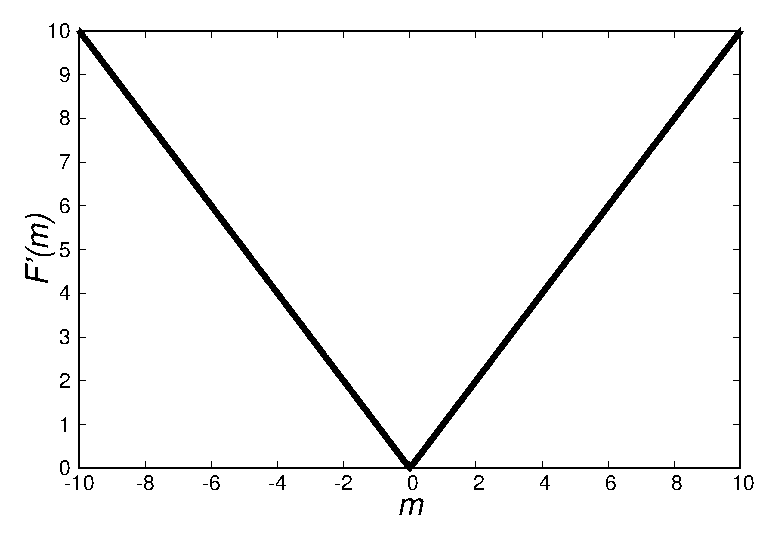
\includegraphics[keepaspectratio,scale=0.33]{minimum_cost_non_t.eps}
      \end{minipage} \\
      \begin{minipage}{0.50\hsize}
        \centering
        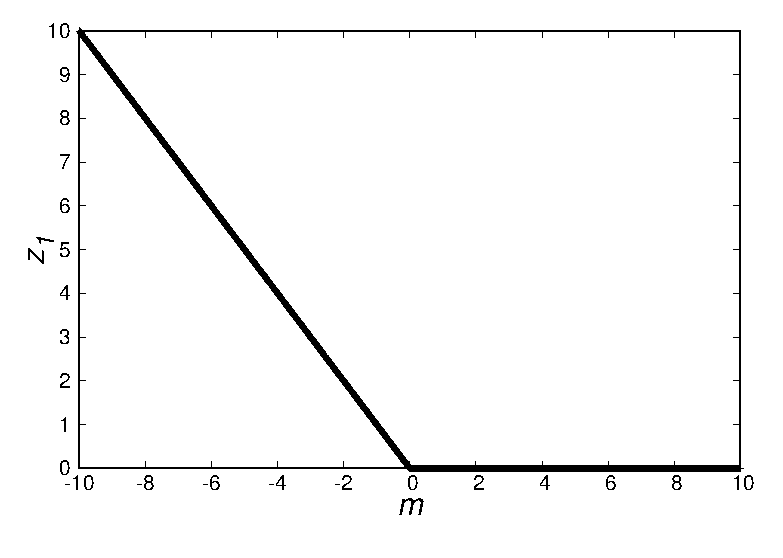
\includegraphics[keepaspectratio,scale=0.33]{minimum_z1_non_t.eps}
      \end{minipage}
      \begin{minipage}{0.50\hsize}
        \centering
        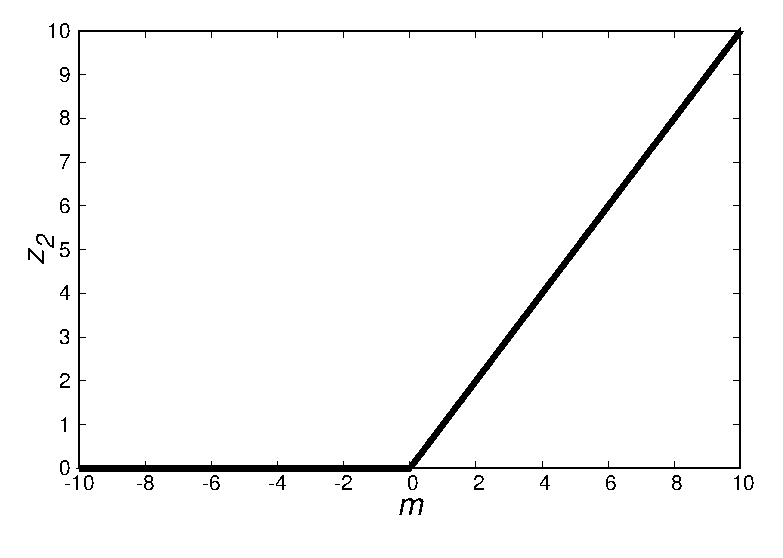
\includegraphics[keepaspectratio,scale=0.33]{minimum_z2_non_t.eps}
      \end{minipage}
    \end{tabular}
    \begin{minipage}{0.03\hsize}
      \vspace{2mm}
    \end{minipage}
    \caption{Numerical results for the simplified QUBO expression in Eq.~\eqref{review_formulation}.
    }
    \label{fig:minimum2}
  \end{center}
\end{figure}

%(大久保)この節全体を以下のように変えてみては?

In order to check the validity of the simplified QUBO formulation in Eq.~\eqref{review_formulation}, we again perform numerical experiments. 
The same settings and procedures as the previous section is employed for the annealing, except for the absence of the variable $t$.
Figure~\ref{fig:minimum2} shows the numerical results; 
it clarifies that the simplified QUBO formulation works well.


\section{Concluding remarks}
%(大久保)節のタイトルを変えました。オリジナルは「conclusion」で、最初が小文字でしたし・・。

%(大久保)全体的に、主張を強くするために書き足しました。素朴にReLUを使うと変数6個で、でもそれが3つになり、さらに2つになる。それは重要、という話ですね。あと、これは書かなくてもいいのですが、Legendre変換で導入された変数 t が不要だったわけですが・・となると、Legendre変換そのものは必要だったんでしょうか?という疑問も・・。ぱっと考えると、必要だったように思うのですが、どうなんでしょうね・・。自明ではないので、そのあたりも、少し主張を強くするために書いておきました。

In this paper, the QUBO formulation for the $\ell_{1}$-norm is derived.
As discussed in Introduction, there is no systematic way to derive the QUBO formulation.
There are some works for the QUBO formulation, and actually that of the ReLU-type function gives the QUBO formulation for the $\ell_{1}$-norm, as discussed in Sect.~3.
However, this needs six additional variables; the reduction of additional variables is important for the Ising-type hardware because of the current limitation of spin variables.
Hence, we carefully applied the Legendre transformation and the Wolfe dual theorem to the $\ell_{1}$-norm, which leads to the QUBO formulation in Eq.~\eqref{after_wolf}; this has only three additional variable.
Furthermore, it was clarified that the QUBO formulation for the $\ell_{1}$-norm is achieved with only two additional variables as shown in Eq.~\eqref{review_formulation}.
At first glance, it is difficult to see the connection between the $\ell_{1}$-norm and the final expression in Eq.~\eqref{review_formulation}.
This nontrivial result is the main contribution of the present work, which means that careful derivation is required individually.

As shown in the derivation, the variable $t$, which is introduced via the Legendre transformation, was reduced finally. It is not clear whether the usage of the Legendre transformation is necessary or not; at this stage, the procedure (the Legendre transformation $\to$ the Wolfe dual theorem $\to$ reduction of variables) is straightforward and understandable.
Of course, there could be more suitable derivation methods.
In addition, when the $\ell_{1}$-norm is combined to another cost function in order to make sparse estimation with the Ising-type hardware, it is necessary to add two variables for each estimated value;
the number of additional variables is still large. 
It will be important future works to find further reduction methods for practical problems with large size.

In order to achieve wider use of the annealing hardware, it is important to derive QUBO formulations for various types of cost functions or regularization terms.
The present work revealed the Legendre transformation, the Wolfe dual theorem, and the careful variable reduction work well for the derivation, and hence we believe that the procedure will be beneficial for future researches on the QUBO formulations and the annealing hardwares.


\begin{acknowledgment}

%\acknowledgment

%For enveironments for acknowledgment(s) are available: \verb|acknowledgment|, \verb|acknowledgments|, \verb|acknowledgment|, and \verb|acknowledgments|.

\end{acknowledgment}

%\appndix
%\section{}
%Use the \verb|\appendix| command if you need an appendix(es). The \verb|\section| command should follow even though there is no title for the appendix (see above in the source of this file).
%For authurs of Invited Review Papers, the \verb|profile| command si prepared for the author(s)' profile. A simple example is shown below.

%\begin{verbatim}
%\profile{Taro Butsuri}{was born in Tokyo, Japan in 1965. ...}
%\end{verbatim}

\begin{thebibliography}{1}
% 統一しましょう。First name を省略で書きます。
\bibitem{d-wave01}
  M. W. Johnson, M. H. S. Amin, S. Gildert, T. Lanting, F. Hamze, N. Dickson, R. Harris, A. J. Berkley, J. Johansson, P. Bunyk, E. M. Chapple, C. Enderud, J. P. Hilton, K. Karimi, E. Ladizinsky, N. Ladizinsky, T. Oh, I. Perminov, C. Rich, M. C. Thom, E. Tolkacheva, C. J. S. Truncik, S. Uchaikin, J. Wang, B. Wilson and G. Rose, Nature {\bf 473}, 194 (2011).
\bibitem{d-wave02}
  P. I. Bunyk, E. Hoskinson, M. W. Johnson, E. Tolkacheva, F. Altomare, A. J. Berkley, R. Harris, J. P. Hilton, T. Lanting, J. Whittaker, IEEE Trans. Appl. Supercond. {\bf 24}, 1700110 (2014).
\bibitem{DA}
  M. Aramon, G. Rosenberg, E. Valiante, T. Miyazawa, H. Tamura, and H. G. Katzgraber, arXiv:1806.08815.

% basics for quantum annealing
\bibitem{Kadowaki1998}
T. Kadowaki and H. Nishimori, Phys. Rev. E {\bf 58}, 5355 (1998).
\bibitem{Farhi2001}
E. Farhi, J. Goldstone, S. Gutmann, J. Lapan, A. Lundgren, and D. Preda, Science {\bf 292}, 472 (2001).

% recent application
\bibitem{Tanahashi2019}
K. Tanahashi, S. Takayanagi, T. Motohashi, and S. Tanaka, J. Phys. Soc. Jpn. {\bf 88}

\bibitem{Biamonte}
J. Biamonte, P. Wittek, N. Pancotti, P. Rebentrost, N. Wiebe and S. Lloyd, Nature {\bf 549}, 195 (2017).

% review
\bibitem{Lucas2014}
A. Lucas, Front. Phys. {\bf 2}, 5 (2014).


% Logic
\bibitem{Whitfield}
J. D. Whitfield, M. Faccin, and J. D. Biamonte, Europhys. Lett. {\bf 99}, 57004 (2012).


\bibitem{black-hole}
% 論文タイトルは引用しないので、統一しましょう。あと [1] で大量の名前を書いているので、こっちも et al. で省略せずに書きましょう。
%  Mareki Honma et al, Imaging black holes with sparse modeling, J.Phys.: Conf. Ser. {\bf 699} 012006 (2016).
  M. Honma, K. Akiyama, F. Tazaki, K. Kuramochi, S. Ikeda, K. Hada, and M. Uemura, J.Phys.: Conf. Ser. {\bf 699} 012006 (2016).

\bibitem{q-loss}
  V. Denchev, N.Ding, S. V. N Vishwanathan, and H. Neven, in Proceedings of the 29th International Conference on Machine Learning, p.863 (2012).

\bibitem{relu}
% すでに出版されているので、arXivではなくて論文を引用しましょう・・。
  G. Sato, M. Konoshima, T. Ohwa, H. Tamura, and J. Ohkubo, Phys. Rev. E {\bf 99}, 042106 (2019).

\bibitem{wolfe}
  P. Wolfe, Quart. Appl. Math. {\bf 19}, 239 (1961).
\bibitem{lasso}
% これもタイトル不要。あと、書式の統一。(1)などは Issue番号で、他の文献にもありますが、記載していないので、ここも記載せず、で。あと、ページ番号も他の引用では冒頭のしか書いていないので、それに統一。
%  Robert Tibshirani, Regression Shrinkage and Selection via the Lasso, J. R. Statist. Soc, B, 58(1):267-288 (1996).
  R. Tibshirani, J. R. Statist. Soc, B {\bf 58}, 267 (1996).
  
\end{thebibliography}

\end{document}

